\section{Drehzahlmessung}
\label{sec:RPM}
Die individuelle Drehzahl aller vier Räder des Modellautos soll erfasst werden. Dafür sind die Auswahl verschiedener Sensortechnologien, die Konstruktion, Fertigung und Montage der Halterungen sowie die Programmierung des Einplatinencomputers notwendig.

\subsection{Wahl der Sensortechnologie}
\label{subsec:RPMchoice}
Aufgrund des Hinterradantriebes des Modellautos sind für die vorderen und hinteren Räder unterschiedliche Sensortypen erforderlich. Durch die Federung des Fahrgestells und der Lenkung der Vorderräder, kommen einige Herausforderungen bei der Sensorwahl und Montage auf. Die Drehzahlerfassung der Hinterräder erfolgt deswegen direkt an den Radantriebswellen des Differentials. Bei den Vorderrädern muss die Drehzahl an den Rädern gemessen werden, da diese nur mitlaufen und keine Welle aufweisen.

\subsubsection{Sensortechnologie der Hinterräder}
\label{subsubsec:RPMchoiceRear}
Für die Drehzahlmessung der Hinterräder werden Infrarot-Gabellichtschranken, wie in Sektion \ref{subsec:tIR} beschrieben, verwendet. Diese geben die Versorgungsspannung von +3.3 V aus, wenn der \ac{IR}-Strahl unterbrochen wird. Auf der zu messenden Welle ist folglich eine Rotationsscheibe anzubringen, welche den \ac{IR}-Strahl periodisch unterbricht. Über die Zeit, die zwischen den einzelnen Unterbrechungen vergeht, lässt sich dann die Drehzahl ermitteln.

\subsubsection{Sensortechnologie der Vorderräder}
\label{subsubsec:RPMchoiceFront}
Wie bereits erwähnt ist es nur möglich, die Drehzahl der Vorderräder direkt am Rad zu erfassen. Eine Möglichkeit dafür wäre es, ebenfalls \ac{IR}-Sensoren zu verwenden. Hier wäre eine Ausführung mit parallel platziertem Sender und Empfänger, anstatt gegenüberliegend, notwendig. Auf diese Art und Weise kann eine schwarze Scheibe am Rad fixiert werden, welche weiße Segmente aufweist. Diese Segmente reflektieren den \ac{IR}-Strahl bei jeder Vorbeibewegung am Sensor. Dadurch kann wieder über die Zeit, die zwischen den Reflexionen vergeht, die Drehzahl ermittelt werden. Unter Berücksichtigung der Nachteile von \ac{IR}-Sensoren und dem Einbauort an den Vorderrädern, treten mehrere potentielle Probleme auf. Zum einen wäre es möglich, dass das Sonnenlicht mit dessen \ac{IR}-Anteil, vom Empfänger des Sensors fälschlicherweise erkannt wird. Bei den Vorderrädern ist die Montageposition relativ offen, wodurch ein direkter Einfall von Außenlicht möglich wäre. Aufgrund dieser ungeschützten Lage, wäre es auch denkbar, dass zum Beispiel Staub oder feiner Sand am Sender, beziehungsweise Empfänger, des \ac{IR}-Sensors haften bleibt und diesen funktionsunfähig macht.\\
Eine robuste und zuverlässige Lösung für die Drehzahlerfassung der Vorderräder sind digitale Hall-Sensoren, eine Erklärung zum Funktionsprinzip von diesen kann in Sektion \ref{subsec:tHall} gefunden werden. Um diese implementieren zu können wird ebenfalls eine Scheibe an der Innenseite der Räder montiert, welche allerdings Permanentmagneten aufweist.


\subsection{Montage der Drehzahlsensoren}
\label{subsec:RPMmount}
Um die Sensoren sowie die Rotationsscheiben zu montieren sind diese zu konstruieren, mit einer gängigen 3D-Druck Methode zu fertigen und anschließend an einer geeigneten Stelle am Auto zu fixieren. Außerdem muss ein System zur Mikrocontroller-Einbindung gewählt und umgesetzt werden.

\subsubsection{Sensormontage der Hinterräder}
\label{subsubsec:RPMmountRear}
Die Drehzahlerfassung der Hinterräder erfolgt an den Radantriebswellen des Differentials, worauf jeweils ein Ring mit vier länglich ausgeführten Extrusionen angebracht ist, wodurch der \ac{IR}-Strahl vier Mal pro Umdrehung unterbrochen wird (Siehe Abbildung \ref{fig:RPMrearDisc}). Um den \ac{IR}-Sensor zu montieren, wird eine spezielle Halterung mithilfe von \ac{CAD} konstruiert. Diese wird mit dem in Sektion \ref{subsec:tDUP} beschriebenen \ac{DUP}-Verfahren gefertigt. Dazu wird ein spezielles mechanisch bearbeitbares Harz verwendet, welches es ermöglicht, unter anderem Gewinde in dementsprechende Bohrungen zu schneiden. Der Sensor wird dann mit einer M3-Schraube mit der Halterung verbunden. Die Halterung selbst wurde so konstruiert, dass sie mit einem Teil des Autos über Formschluss sowie zwei Schrauben fixiert wird, wie es in Abbildung \ref{fig:RPMrearMount} veranschaulicht wird.
\begin{figure}[h]
\centering
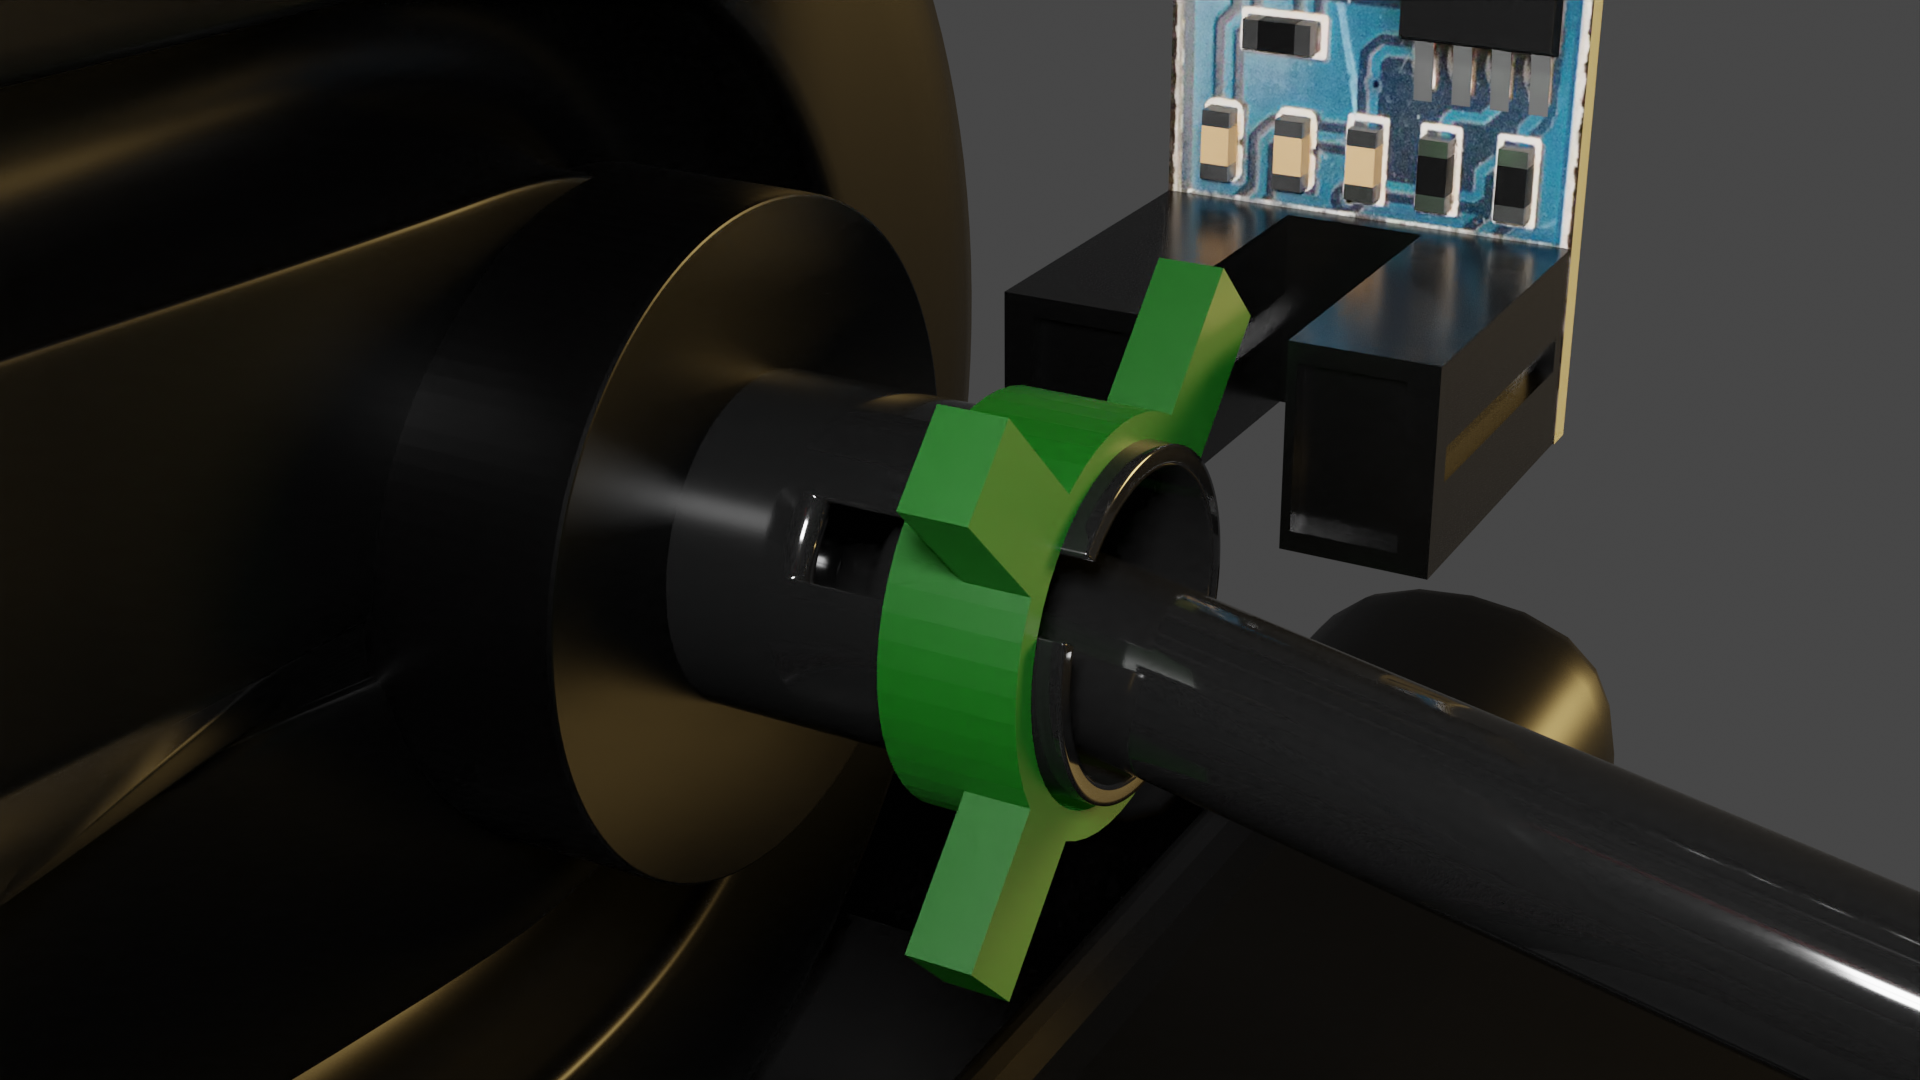
\includegraphics[scale=0.2]{RPMrearDisc.png}
\caption{Rotationsring zur Drehzahlmessung (zur Veranschaulichung grün)}
\label{fig:RPMrearDisc}
\end{figure}

\begin{figure}[h]
\centering
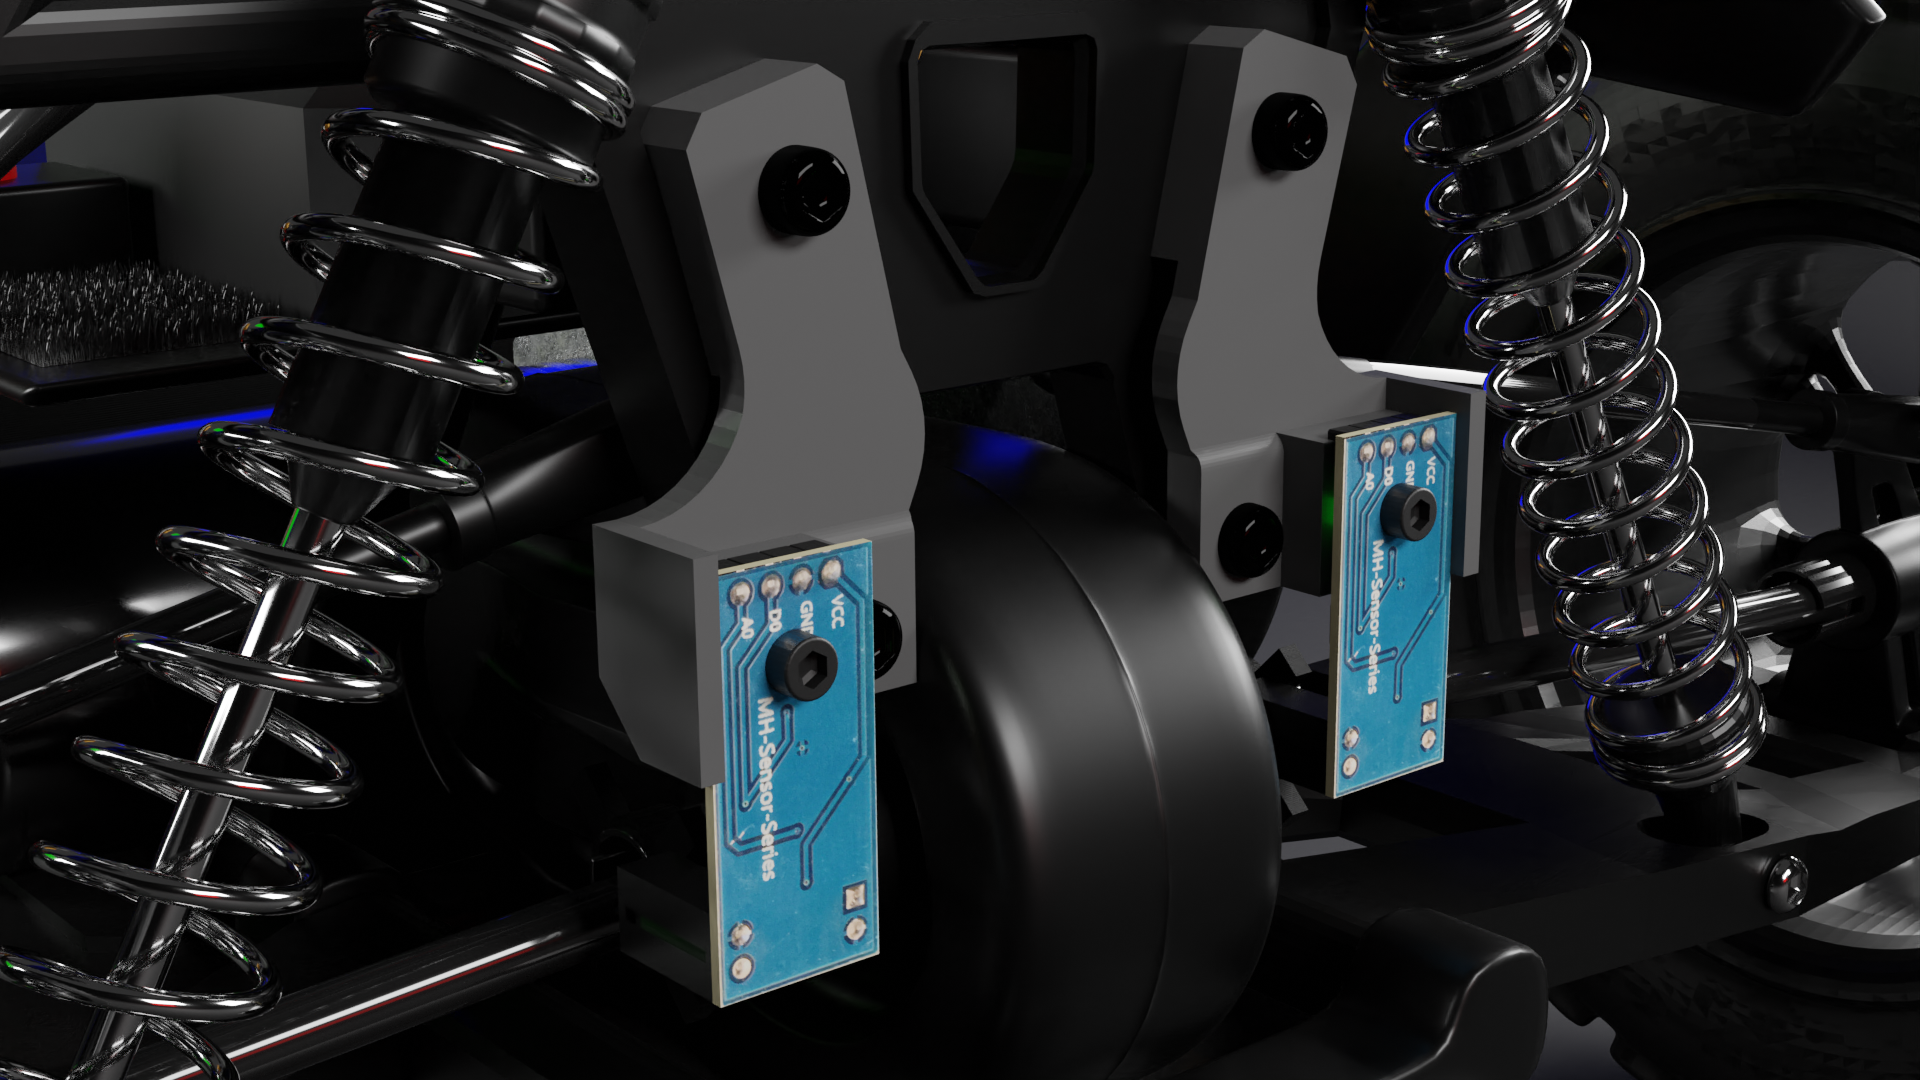
\includegraphics[scale=0.2]{RPMrearMount.png}
\caption{Montage der \ac{IR}-Sensoren}
\label{fig:RPMrearMount}
\end{figure}

\subsubsection{Sensormontage der Vorderräder}
\label{subsubsec:RPMmountFront}
Wie bereits erwähnt, erfolgt die Messung der Vorderrad-Drehzahl an den Rädern direkt. An der Innenseite dieser, ist eine Scheibe mit vier eingelassenen Permanentmagneten angebracht, wodurch der Hall-Sensor pro Umdrehung vier Mal ausschlägt. Der Sensor selbst muss am selben Bauteil befestigt werden, woran auch das Rad befestigt ist. Nur so kann eine Messung erfolgen, da durch die Lenkung und Federung der Räder die Position der Scheibe relativ zum Sensor nicht konstant wäre. Die Halterung für den Sensor sowie die Scheibe, wurden mithilfe von \ac{CAD} konstruiert und anschließend mit dem in Sektion \ref{subsec:tFDM} beschriebenen \ac{FDM}-Verfahren gefertigt. Die Dauermagneten sind in die Einlassungen auf der Scheibe eingeklebt und die Scheibe selbst ist ebenfalls per Verklebung an der Radinnenseite befestigt. Der Hall-Sensor ist mit einer M3-Schraube an der Halterung fixiert und die Sensorhalterung ist mit zwei weiteren Schrauben montiert. Eine robuste Verbindung des Sensors ist aufgrund der Bewegungen des Lenksystems und der Federung und somit der Sensoren, besonders wichtig.

\begin{figure}[h]
\centering
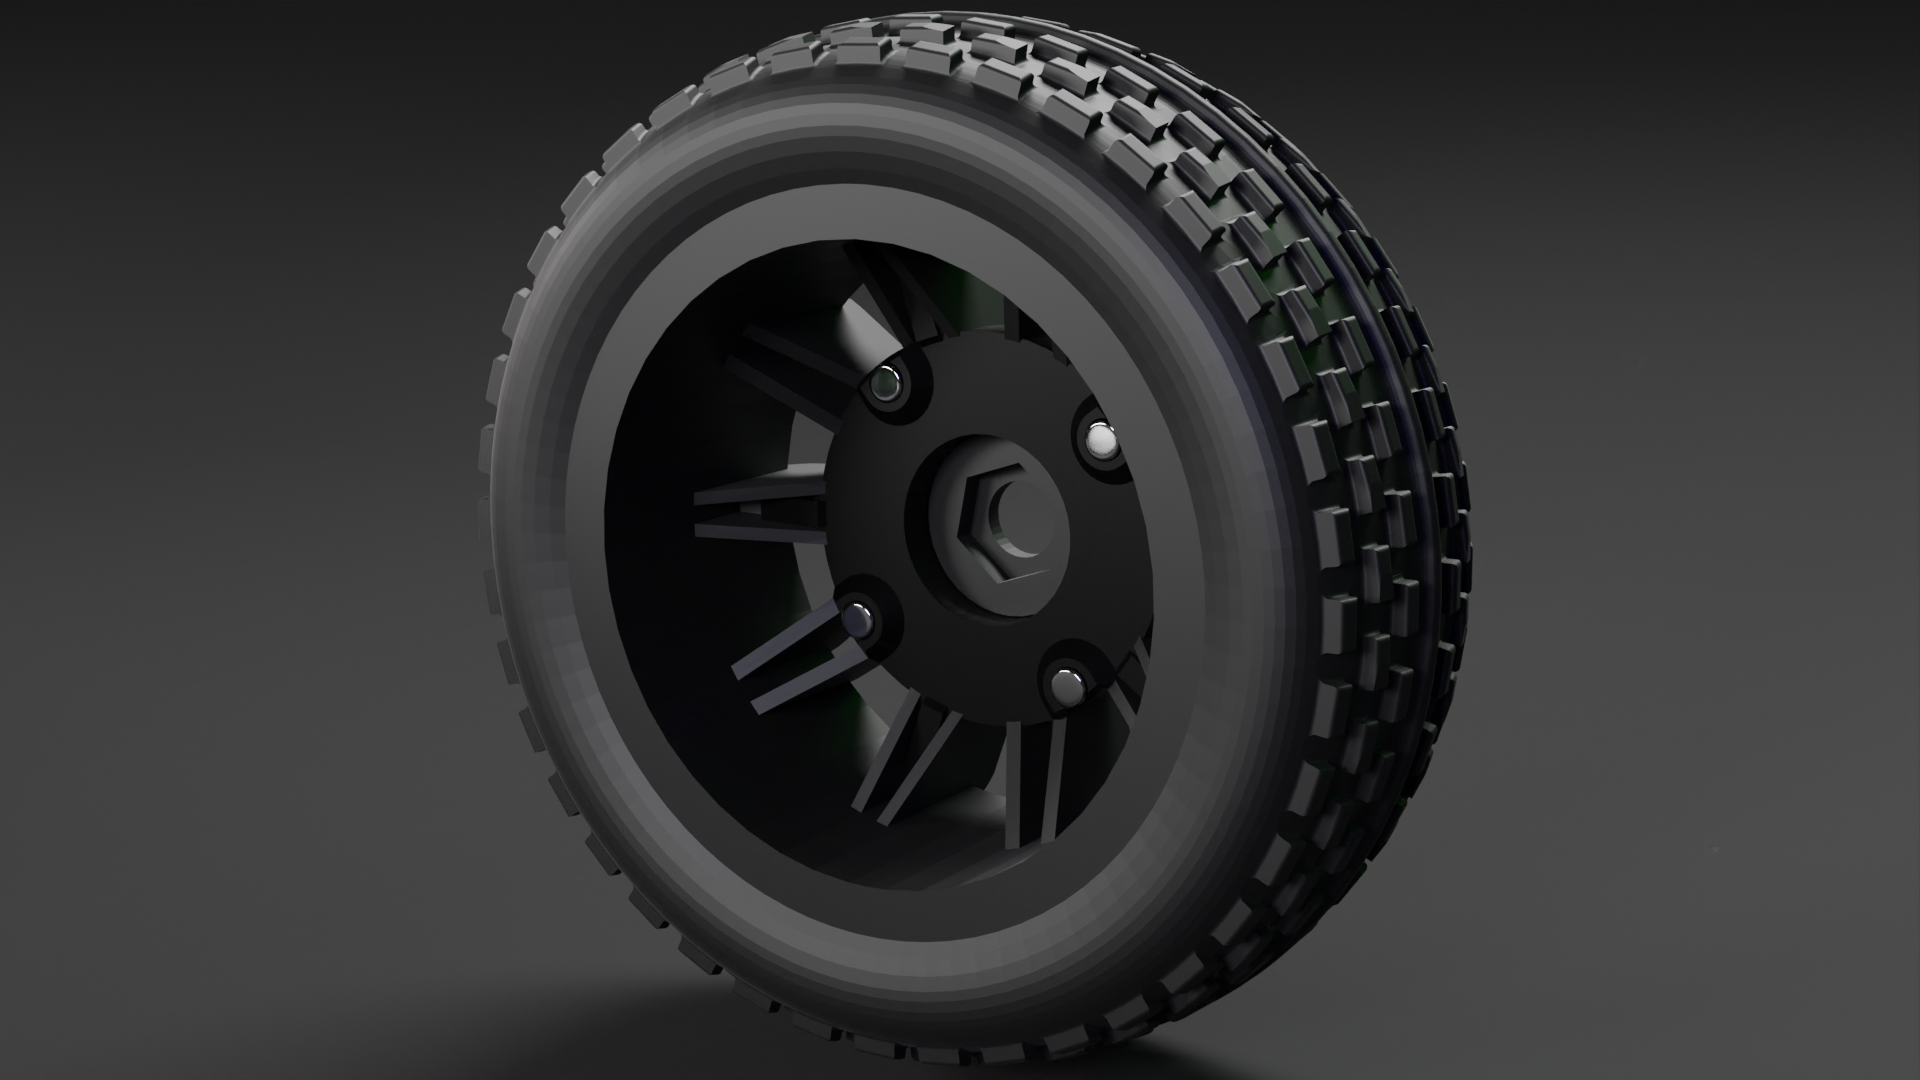
\includegraphics[scale=0.2]{RPMfrontDisc.png}
\caption{Rotationsscheibe mit Dauermagneten in Vorderrad}
\label{fig:RPMfrontDisc}
\end{figure}

\begin{figure}[h]
\centering
\missingfigure{}
\caption{Montage der Hall-Sensoren}
\label{fig:RPMfrontMount}
\end{figure}

\subsection{Programmatische Implementation der Drehzahlsensoren}
\label{subsec:RPMprogram}
Die \ac{IR}- sowie die Hall-Sensoren liefern prinzipiell ein Rechtecksignal. Eine steigende Flanke entspricht dabei einer Unterbrechung des Magnetfeldes, beziehungsweise einer Erkennung des Magnetfeldes. Die Zeit, die zwischen den steigenden Flanken vergeht, ist  die Zeit, die für ein Viertel einer Umdrehung des Rades benötigt wird. Mit steigender Drehzahl nimmt diese Zeit somit ab und die Periodendauer des Signals wird kürzer. Die Signalleitung der Drehzahlsensoren ist an den \ac{GPIO}-Pins des Raspberry Pi angeschlossen. Somit kann mithilfe eines Interrupts eine steigende Flanke an so einem \ac{GPIO}-Pin erkannt werden, wodurch es möglich ist, die Zeit seit der letzten steigenden Flanke festzuhalten.\\
Ein Interrupt ist eine Unterbrechung des normalen Ablaufs des Programmes, woraufhin eines sogenannte Interrupt-Serviceroutine, auch callback genannt, ausgeführt wird. Dieser Interrupt kann zum Beispiel über eine Zustandsänderung an diesen \ac{GPIO}-Pins ausgelöst werden. Für die Erfassung der Drehzahl werden für jeden Sensor, also insgesamt vier dieser Interrupts erstellt. Diese erfassen eine steigende Flanke der Drehzahlsensoren und führen die callback Routine für den jeweiligen Sensor aus. In dieser wird zunächst die aktuelle Zeit, mithilfe der in Sektion \ref{subsubsec:tLibTime} beschriebenen Bibliothek time, auf eine Variable geschrieben. Die Differenz der letzten Zeit und der Aktuellen wird anschließend berechnet. Danach wird für den nächsten Routineaufruf die aktuelle Zeit auf die Variable der vorherigen \glqq alten\grqq\ Zeit geschrieben.\\
Aus dieser Zeitdifferenz wird die Drehzahl errechnet. Dazu wird zunächst der Kehrwert dieser Zeit berechnet, was im Grunde genommen direkt einer Drehzahl entspricht. Dieser Wert wird mit 60 multipliziert um die Einheit $\frac{1}{min}$ zu erhalten. Da die umgerechnete Zeit allerdings für eine Viertelumdrehung gilt, muss das Ergebnis durch vier dividiert werden.
\begin{equation}
rpm=\frac{\frac{60}{\Delta time}}{4}
\label{eqn:rpm}
\end{equation}
\\
Aus dieser Berechnungsmethode geht jedoch das Problem hervor, dass bei einer fehlerhaften Erkennung der Sonneneinstrahlung als Ende der Unterbrechung des \ac{IR}-Lichtstrahles an den Gabellichtschranken eine stark verfälschte Drehzahl in diesem Datensatz auftreten kann, wenn diese Einstrahlung im falschen Moment geschieht. Um einen solchen Fehler zu kompensieren wird zusätzlich zur oben beschriebenen Berechnungsmethode auch noch eine separate Methode verwendet, welche dieses Problem nicht aufweist. Bei dieser alternativen Berechnungsmethode wird pro Unterbrechung ein Zähler um Eins erhöht, die Zeit zwischen den Berechnungsvorgängen gemessen und nach der Berechnung der Zähler zurückgesetzt.
\begin{equation}
rpm_{alt}=\frac{\frac{cnt}{\Delta time}\cdot 60}{4}
\label{eqn:altrpm}
\end{equation}

Gilt also $rpm > rpm_{alt} \cdot 1.5$, wird statt der normalen Berechnung die alternative Berechnung verwendet, da dann die Chance, dass die Sonneneinstrahlung die Messwerte manipuliert hat zu hoch ist, um die genauere, primäre Berechnungsart zu verwenden.\\\\
Zusätzlich wird aus den Drehzahlen der Räder die Geschwindigkeit des Fahrzeuges errechnet. Dazu wird der Durchmesser der Vorderräder in Metern mit $\pi$ und dem Mittelwert der Drehzahl der Vorderräder in Umdrehungen pro Sekunde multipliziert. Das Ergebnis ist die Fahrgeschwindigkeit in Metern pro Sekunde.
\begin{equation}
v=D_{Wheel}\cdot\pi\cdot\frac{n_{WheelR}+n_{WheelL}}{2}
\label{eqn:velocity}
\end{equation}


